\chapter{Results}\label{ch:results}

From the experiments described in chapter \ref{ch:experiments} a framework was created and tested in chapter \ref{ch:method}. 
The 'easy to use' tools like iPerf3, hping and BoNeSi are useful for quick tests. But when it comes to representative session based application testing these tools do not offer the solution for high speed networks. 
As these 'easy to use' tools all require the kernel to talk to the hardware. As described in section \ref{sub:dpdk}, DPDK is able to bypass the kernel and talk to the interface directly. Cores and memory needs to be dedicated to generate traffic.  

\section{Infrastructure}
The network at 'company x' as it is shown in figure \ref{fig:testenv} is a simplified representation.
The detailed infrastructure used during the real world test is displayed in figure \ref{fig:companyx} 
Since all the network hardware is redundant and a single device failures cannot result in a total downtime the figure and therefore the monitoring gets more complicated.
The server is connected to a data center layer that is spread over two physical locations, one serving as the active and the other as the passive environment.
To minimize the unnecessary traffic between the data centers an overlay technique is used. This overlay also blocks broadcast storms at one location spreading to the other location.  
When traffic does not arrive at the destination, detailed measurements are needed at every device for every link to determine where the traffic gets dropped.   

\begin{figure}[H] 
  \includegraphics[scale=0.4]{images/companyx.pdf}
  \caption{Detailed visualization of real world scenario.}
  \label{fig:companyx}
\end{figure}

\section{Data Plane Development Kit based tools}
Since none of the use cases require the 'easy to use' tools, simply due to the fact that these tools do not reach the performance required for this research. 
The results of the DPDK based applications are explained during the use case performance tests on the real world scenario.
  
\subsection{pktgen}
Pktgen was used to get the limitations from the test hardware: It was already known that the maximum amount of pps is a hardware limitation inside the PCI Express Bus. 
The maximum link speed can be reached when packets of 400 bytes are used. To get an idea of the throughput over the entire path from client to server, pktgen is used to setup a UDP stream from the client to the server. 
The source IP address and port towards the destination IP address and port are the same. Since aggregated interfaces are used from the test switch to the router, the hashing algorithm in the switch limits the traffic to only one link filled up by this test. 
Figure \ref{fig:surftest} shows a maximum throughput of 7 Gb/s at 20:40. This was transported to company x and delivered to router1, the logical aggregation of the physical routers 1a and 1b. From here it is important to know what lines are used to transport the traffic towards the firewall.
Figures \ref{fig:testrealusageae112} and \ref{fig:testrealusageae113} display the graphs of the traffic that went out of the aggregated interfaces connecting router1 to the firewall cluster and the links connecting the firewalls to the DCI switches inside the data center. The white gaps between send and received data, is traffic that got lost during the execution of the use cases. Data points above zero represent data that went from server to client and data points below zero represent data from client to server. 
   
\begin{figure}[H]
  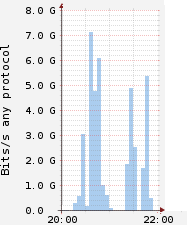
\includegraphics[scale=0.5]{images/test-link-usage.png}
  \caption{Bandwidth utilization of real world tests during the time window of the tests.}
  \label{fig:surftest}
\end{figure}

\begin{figure}[H]
  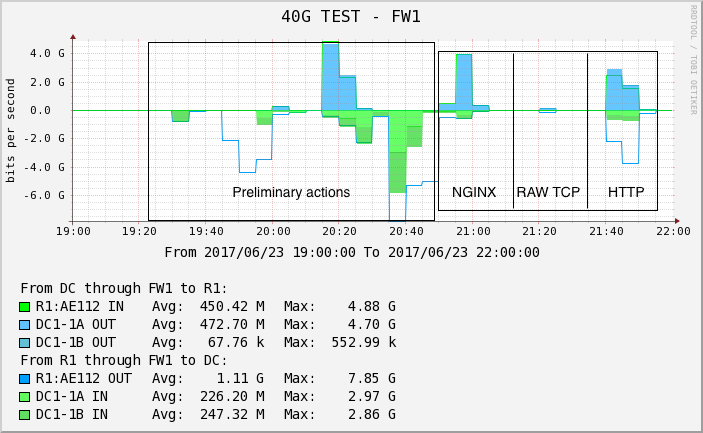
\includegraphics[scale=0.5]{images/real-ae112.png}
  \caption{Bandwidth utilization of links between router1, firewall1 and DC1 during the time window of the tests, spikes represent an executed test.}
  \label{fig:testrealusageae112}
\end{figure}

\begin{figure}[H]
  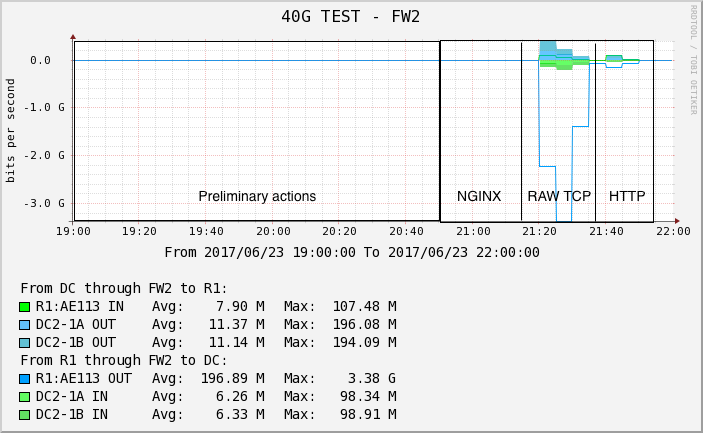
\includegraphics[scale=0.5]{images/real-ae113.png}
  \caption{Bandwidth utilization of links between router1, firewall2 and DC2 during the time window of the test, the spike represents the moment of a fail over to the secondary machine.}
  \label{fig:testrealusageae113}
\end{figure}



% 20:42 - 20:50 PKTGEN UDP en TCP
% 20:54 - 21:00 WARP - NGINX
% 21:21 - 21:30 WARP - RAW TCP
% 21:42 - 22:00 WARP - HTTP

\subsection{WARP}
From the benchmark results performed on WARP in chapter \ref{ch:experiments} it is known WARP is capable of generating almost a million sessions per second. 
WARP was used to run three tests. WARP needs to be commanded using its own syntax. The command file that was used for the NGINX server test and the WARP HTTP server test can be found in appendix \ref{appendix:software}. As WARP runs on top of DPDK, the DPDK commands point to resources that will be claimed by DPDK. As an example:

\begin{verbatim}
./build/warp17 -c ff -n 4 -m 32768 -- --qmap-default max-c \
--ucb-pool-sz 32768 --tcb-pool-sz 32768 --cmd-file \
test-client-nginx-http.txt 
\end{verbatim} 

Figure \ref{fig:warptime} shows the results of the three experiments. 
Therefore, WARP was used to retrieve a 500 Kbyte file from an NGINX web server running on server A.
The file was placed on a RAM disk to make sure disk IO would not be the bottleneck during the performance tests. 
This test is executed starting at 20:50 and it ran until 21:00. The request size is increased every 90 seconds with an interval of 30 seconds between the tests.
During this test the following request sizes where used: 64, 256, 512, 1024 and 2048 bytes. 
Figure \ref{fig:realnginx} shows that the amount of traffic leaving the server goes above 4Gb while only 0.6 Gb of requests are coming in on the receiving end. 
This matches the values shown in figure \ref{fig:testrealusageae112}. \\
Rate limiting at the NGINX server on the receiving end (allowing the server to accept a maximum of 40 thousand concurrent sessions) made sure nothing broke. The services got depleted at the machine, this made the service unavailable for other users.
The graphs show us that traffic was not lost during this test.

\begin{figure}[]
  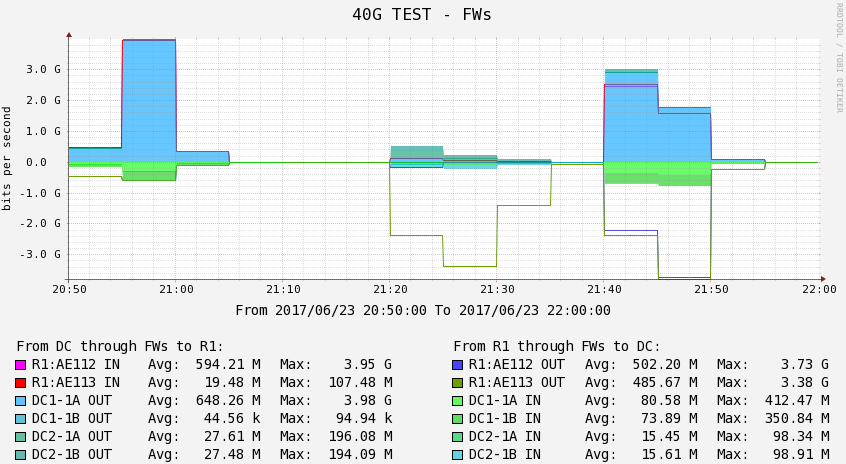
\includegraphics[scale=0.5]{images/warp-timeline.png}
  \caption{Time line of the preformed tests using WARP displaying the bandwidth usage over time}
  \label{fig:warptime}
\end{figure}

\begin{figure}
  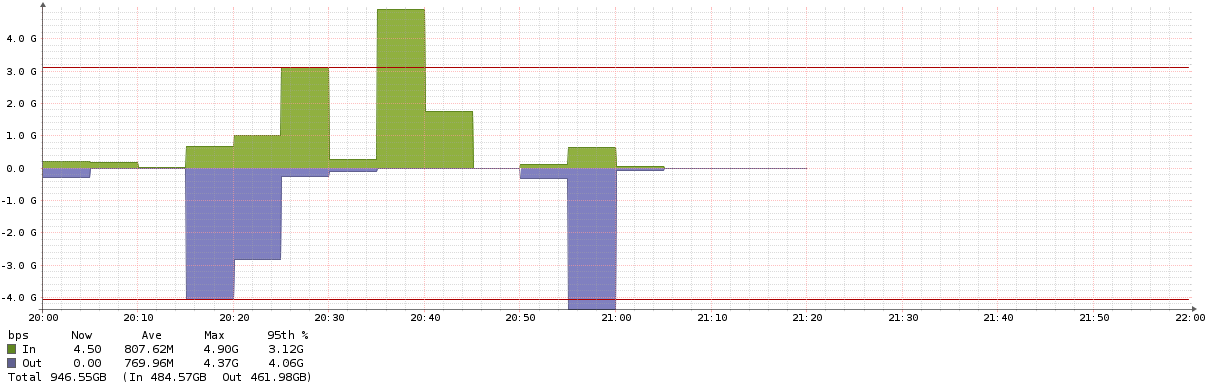
\includegraphics[scale=0.35]{images/real-nginx.png}
  \caption{Bandwidth utilization server A during NGINX test, measurements from servers perspective }
  \label{fig:realnginx}
\end{figure}


At 21:20 the next test was started, generating a maximum amount of RAW TCP sessions (this test is performed on OSI layer 4 by sending TCP RAW request and responses) from client to server both running WARP and using 32GB of memory and all cores to generate traffic.
Request and response sizes chosen for this tests are: 64, 256, 512, 1024 and 2048 bytes. 
Since WARP needs control of the interfaces, the server's kernel will not display any traffic on the interfaces. 
The measurements all came from the uplink and downlink interfaces of the devices in the path as shown in figure \ref{fig:companyx} represented by "AE112" and "AE113"
Sessions statistics where not registered due to logging problems in the firewall environment. 
Chapter \ref{ch:experiments} shows that the benchmark value of 1 million sessions per second is generated, no differences are observed at different packets sizes. 
Only 10\% of the link is utilized at the starting point of the benchmark test as displayed in \ref{fig:rawtcplink}. 
The graph in figure \ref{fig:testrealusageae112} doesn't display any traffic at 21:20. This is the moment the RAW TCP test was started while figure \ref{fig:surftest} displays traffic towards the tested network. 
The graph in figure \ref{fig:testrealusageae113} displays the load. When the test started, the active firewall crashed and a failover to the passive machine is the result. Log messages retrieved from connected routers also display BGP session failures from the formerly-active firewall. 
This graph also displays the difference between traffic send from the router to the firewall and the traffic received by the downstream switch. 
Input is 3Gb and output is in the range of 200 - 300 Mb. The firewall had a rule accepting all the traffic from the source range of the test machines.
The firewalls are not capable of handling this amount of sessions per second. Due to time limitations this test could not be performed again to figure out the limitations.  
When the test was finished, the firewalls started to recover. \\ 

The firewall environment was restored to the way it was in the beginning of the first test.
At 21:40 the last test is started between server and client, again both running WARP. Generating the maximum amount of HTTP sessions using 32GB of memory and all available cores.
Generating a GET request and responding with a 200-(OK) message from the server running WARP instead of NGINX.  
From the experimental phase of this research it is known that WARP is capable of handling more request per second than NGINX can. This last test is executed to find the limits of intermediate hardware when HTTP sessions are opened up in a fast rate.
Message sizes for the tests are : 64, 256, 512, 1024 and 2048 bytes. Request and response size are equal. 
With the information from the benchmark in chapter \ref{ch:experiments} the limitations of client and server are known. 
From the tests at 21:20 it is known the firewalls will die when to many sessions per second come in. The same behavior is expected during this test.
Figure \ref{fig:testrealusageae112} shows 4Gb/s going into the firewall and only 500Mb/s of HTTP traffic arriving at the other side.
This means that the firewall was not able to handle the amount of sessions per second and the machines stop functioning. 
Management sessions broke down and traffic got lost.


